\documentclass[11pt,a4paper]{article}

\usepackage[a4paper,margin=1in]{geometry}
\usepackage{amsmath}
\usepackage{booktabs}
\usepackage{array}
\usepackage{enumitem}
\usepackage{tikz}
\usepackage{fancyhdr}
\usepackage[T1]{fontenc}
\usepackage{lmodern}

\usetikzlibrary{positioning}

\newcommand{\universityname}{UNIVERSITY OF DERBY}
\newcommand{\college}{College of Science and Engineering}
\newcommand{\examtitle}{Practice Paper A Solutions}
\newcommand{\moduletitle}{OPERATIONAL RESEARCH}
\newcommand{\modulecode}{5CM522}

\pagestyle{fancy}
\fancyhf{}
\fancyfoot[C]{\thepage}
\renewcommand{\headrulewidth}{0pt}

\setlength{\parindent}{0pt}
\setlength{\parskip}{0.45em}
\setlist[enumerate,1]{label=(\alph*), leftmargin=1.1cm, itemsep=0.4em, topsep=0.3em}

\begin{document}

\begin{center}
{\large \textbf{\universityname}}\\
{\college}\\[0.4em]
{\Large \textbf{\examtitle}}\\
{\large \textbf{\moduletitle} -- \textbf{\modulecode}}
\end{center}

\textbf{1. Linear Programming}

Let $D$ be desks and $S$ be shelving units.

\begin{enumerate}
\item A suitable model is
\[
\max Z = 58D + 46S
\]
subject to
\[
5D + 3S \le 120
\]
\[
2D + 4S \le 96
\]
\[
S \ge 8
\]
\[
D,S \ge 0
\]

\item At the optimum, carpentry and finishing are both binding:
\[
5D+3S=120,\qquad 2D+4S=96
\]
Hence
\[
D=\frac{96}{7}\approx 13.71,\qquad S=\frac{120}{7}\approx 17.14
\]
Maximum contribution:
\[
Z=58D+46S=1584
\]

\item Binding constraints: carpentry and finishing.

Slack values:
\[
5D+3S=120 \Rightarrow 0 \text{ carpentry slack}
\]
\[
2D+4S=96 \Rightarrow 0 \text{ finishing slack}
\]
\[
S-8=\frac{64}{7}\approx 9.14
\]
So the minimum shelving requirement is not binding.

\item If shelving contribution rises to \pounds52, the objective becomes
\[
\max Z=58D+52S
\]
The optimal corner remains the same:
\[
\left(D,S\right)=\left(\frac{96}{7},\frac{120}{7}\right)
\]
with revised contribution
\[
Z=\frac{11808}{7}\approx 1686.86
\]
So the basis does not change.

\item The new condition is
\[
S \ge 0.3(D+S)
\]
which simplifies to
\[
3D-7S \le 0
\]
At the original optimum,
\[
\frac{S}{D+S}=\frac{17.14}{30.86}\approx 55.6\%
\]
so the original solution remains feasible. The optimal plan is unchanged.
\end{enumerate}

\textbf{2. Binary Integer Programming}

Let $x_A,\ldots,x_F \in \{0,1\}$ where $x_i=1$ if project $i$ is selected.

\begin{enumerate}
\item A suitable model is
\[
\max B = 14x_A+17x_B+11x_C+20x_D+9x_E+15x_F
\]
subject to the budget constraint
\[
6x_A+8x_B+5x_C+9x_D+4x_E+7x_F \le 21
\]
and the logical constraints
\[
x_D \le x_B
\]
\[
x_A+x_F \le 1
\]
\[
x_C+x_E \ge 1
\]
\[
x_i \in \{0,1\}
\]

\item The optimal solution is
\[
x_B=x_D=x_E=1,\qquad x_A=x_C=x_F=0
\]
Total cost:
\[
8+9+4=21
\]
Maximum benefit:
\[
17+20+9=46
\]

\item Binary variables are needed because a project cannot be partly selected in any practical sense. A continuous LP could return fractional values such as ``0.4 of project $D$'', which would not be meaningful here.

\item Add
\[
x_A+x_B+x_C+x_D+x_E+x_F = 4
\]
There is no feasible solution satisfying all rules, the budget and the requirement to choose exactly four projects.

\item Example extension: allow projects to be staged over several years with different annual budgets and inter-year dependencies.
\end{enumerate}

\textbf{3. Minimum Spanning Tree}

\begin{enumerate}
\item A minimum spanning tree connects all nodes at minimum total cost without forming cycles.

\begin{center}
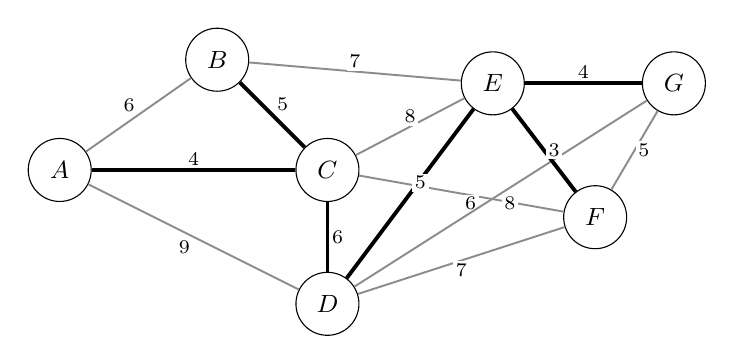
\begin{tikzpicture}[
	depot/.style={circle,draw,minimum size=8mm,inner sep=0pt,font=\small},
	edge label/.style={fill=white,inner sep=1pt,font=\scriptsize},
	nonmst/.style={draw=black!45,line width=0.7pt},
	mst/.style={draw=black,line width=1.4pt}
]
	\node[depot] (A) at (0,2) {$A$};
	\node[depot] (B) at (2,3.4) {$B$};
	\node[depot] (C) at (3.4,2) {$C$};
	\node[depot] (D) at (3.4,0.3) {$D$};
	\node[depot] (E) at (5.5,3.1) {$E$};
	\node[depot] (F) at (6.8,1.4) {$F$};
	\node[depot] (G) at (7.8,3.1) {$G$};

	\draw[nonmst] (A) -- (B) node[midway,above left,edge label] {6};
	\draw[mst] (A) -- (C) node[midway,above,edge label] {4};
	\draw[nonmst] (A) -- (D) node[midway,below left,edge label] {9};
	\draw[mst] (B) -- (C) node[midway,above right,edge label] {5};
	\draw[nonmst] (B) -- (E) node[midway,above,edge label] {7};
	\draw[mst] (C) -- (D) node[midway,right,edge label] {6};
	\draw[nonmst] (C) -- (E) node[midway,above,edge label] {8};
	\draw[nonmst] (C) -- (F) node[midway,below right,edge label] {6};
	\draw[mst] (D) -- (E) node[midway,above right,edge label] {5};
	\draw[nonmst] (D) -- (F) node[midway,below,edge label] {7};
	\draw[nonmst] (D) -- (G) node[midway,below right,edge label] {8};
	\draw[mst] (E) -- (F) node[midway,right,edge label] {3};
	\draw[mst] (E) -- (G) node[midway,above,edge label] {4};
	\draw[nonmst] (F) -- (G) node[midway,right,edge label] {5};
\end{tikzpicture}
\end{center}

\item One correct Kruskal solution selects:
\[
EF(3),\ AC(4),\ EG(4),\ BC(5),\ DE(5),\ CD(6)
\]

\item Total installation cost:
\[
3+4+4+5+5+6=27
\]

\item The cheapest extra non-tree link has cost 5, for example $FG$.

So one cheapest backup addition is $FG$, giving revised total cost
\[
27+5=32
\]

\item Limitation: an MST gives no built-in redundancy, so a single link failure can disconnect part of the network.
\end{enumerate}

\textbf{4. Simulation}

\begin{enumerate}
\item A suitable simulation model would treat weekly deliveries and weekly demand as random inputs. State variables would include opening stock, ending stock and overflow stock. Key outputs would be average weekly cost, overflow frequency and the average size of overflow inventory.

\item One valid 12-week simulation can be produced using seed 2026, giving:

Deliveries:
\[
7,8,8,9,7,7,8,8,9,8,9,9
\]
Demands:
\[
8,7,6,7,5,8,7,8,7,7,6,6
\]

Assume opening stock is 0 and ending stock carries forward week to week.

For capacity 7:

\begin{center}
\begin{tabular}{cccccccc}
\toprule
Week & Open & Delivered & Demand & Sales & End Stock & Overflow & Cost \\
\midrule
1 & 0 & 7 & 8 & 7 & 0 & 0 & 126 \\
2 & 0 & 8 & 7 & 7 & 1 & 0 & 126 \\
3 & 1 & 8 & 6 & 6 & 3 & 0 & 126 \\
4 & 3 & 9 & 7 & 7 & 5 & 0 & 126 \\
5 & 5 & 7 & 5 & 5 & 7 & 0 & 126 \\
6 & 7 & 7 & 8 & 8 & 6 & 0 & 126 \\
7 & 6 & 8 & 7 & 7 & 7 & 0 & 126 \\
8 & 7 & 8 & 8 & 8 & 7 & 0 & 126 \\
9 & 7 & 9 & 7 & 7 & 9 & 2 & 186 \\
10 & 9 & 8 & 7 & 7 & 10 & 3 & 216 \\
11 & 10 & 9 & 6 & 6 & 13 & 6 & 306 \\
12 & 13 & 9 & 6 & 6 & 16 & 9 & 396 \\
\bottomrule
\end{tabular}
\end{center}

\item Total 12-week cost for capacity 7:
\[
2112
\]
Estimated average weekly cost:
\[
\frac{2112}{12}=176.0
\]

\item Using the same 12-week random stream:

\begin{center}
\begin{tabular}{lcc}
\toprule
Capacity & Total Cost & Average Weekly Cost \\
\midrule
6 & 2106 & 175.5 \\
7 & 2112 & 176.0 \\
8 & 2208 & 184.0 \\
9 & 2304 & 192.0 \\
\bottomrule
\end{tabular}
\end{center}

On this run, capacity 6 gives the lowest average weekly cost of \pounds175.5. The other averages are \pounds176.0 for capacity 7, \pounds184.0 for capacity 8 and \pounds192.0 for capacity 9. Therefore, 6 bays appears to be the optimal capacity from this simulation. Increasing capacity beyond 6 raises the fixed bay cost faster than it reduces overflow cost on this run.

\item Two reasons to run a longer or repeated simulation:

The 12-week result may be strongly affected by random variation.

Longer runs or replications would give a more stable estimate of average cost and better evidence for comparing capacities.
\end{enumerate}

\textbf{5. Forecasting}

\begin{enumerate}
\item Using periods 1--12 only, centred 4-quarter moving averages are available for periods 3--10:

\begin{center}
\begin{tabular}{ccc}
\toprule
Period & Demand & CMA \\
\midrule
3 & 570 & 602.25 \\
4 & 690 & 612.25 \\
5 & 548 & 622.25 \\
6 & 662 & 633.50 \\
7 & 608 & 645.25 \\
8 & 742 & 656.25 \\
9 & 590 & 666.75 \\
10 & 708 & 677.75 \\
\bottomrule
\end{tabular}
\end{center}

A linear trend fitted to these centred moving averages is
\[
\hat{T}_t = 568.75 + 10.89t
\]
where $t=1$ corresponds to 2020 Q1.

\item Seasonal indices:

Additive:
\[
Q1=-75.72,\quad Q2=29.16,\quad Q3=-34.97,\quad Q4=81.53
\]

Multiplicative:
\[
Q1=0.8826,\quad Q2=1.0446,\quad Q3=0.9442,\quad Q4=1.1286
\]

\item Validation forecasts for 2023:

\begin{center}
\begin{tabular}{lccc}
\toprule
Quarter & Actual & Additive Forecast & Multiplicative Forecast \\
\midrule
2023 Q1 & 636 & 634.60 & 626.93 \\
2023 Q2 & 760 & 750.36 & 753.38 \\
2023 Q3 & 692 & 697.13 & 691.23 \\
2023 Q4 & 852 & 824.52 & 838.54 \\
\bottomrule
\end{tabular}
\end{center}

Using MAD:
\[
\text{MAD}_{\text{add}} \approx 10.91,\qquad \text{MAD}_{\text{mult}} \approx 7.48
\]
where absolute error is calculated as $|\text{Actual} - \text{Forecast}|$.

For the multiplicative model:
\[
|636-626.93|=9.07,\quad |760-753.38|=6.62,\quad |692-691.23|=0.77,\quad |852-838.54|=13.46
\]
so
\[
\text{MAD}_{\text{mult}}=\frac{9.07+6.62+0.77+13.46}{4}\approx 7.48
\]

For the additive model:
\[
|636-634.60|=1.40,\quad |760-750.36|=9.64,\quad |692-697.13|=5.13,\quad |852-824.52|=27.48
\]
so
\[
\text{MAD}_{\text{add}}=\frac{1.40+9.64+5.13+27.48}{4}\approx 10.91
\]
The multiplicative model is better.

\item Forecasts for 2024 using the multiplicative model:

\begin{center}
\begin{tabular}{lc}
\toprule
Quarter & Forecast \\
\midrule
2024 Q1 & 665.38 \\
2024 Q2 & 798.88 \\
2024 Q3 & 732.35 \\
2024 Q4 & 887.70 \\
\bottomrule
\end{tabular}
\end{center}
\end{enumerate}

\textbf{6. Transhipment}

\begin{enumerate}
\item Use a network flow model with variables defined on the links of the network.

Let the node sets be:
\[
S=\{D_1,D_2,D_3\}, \qquad H=\{H_1,H_2\}, \qquad C=\{C_1,C_2,C_3,C_4\}
\]
and let the arc set be
\[
A=\{(i,h): i \in S,\ h \in H\} \cup \{(h,j): h \in H,\ j \in C\}.
\]

Let
\[
x_{uv}=\text{flow on arc }(u,v)\text{ for each }(u,v)\in A
\]
and let $k_{uv}$ be the corresponding unit transportation cost.

Objective:
\[
\min Z=\sum_{(u,v)\in A} k_{uv}x_{uv}
\]

Supply constraints for each depot $i \in S$:
\[
\sum_{h \in H} x_{ih} \le s_i
\]

Demand constraints for each clinic $j \in C$:
\[
\sum_{h \in H} x_{hj} = r_j
\]

Flow-balance constraints for each hub $h \in H$:
\[
\sum_{i \in S} x_{ih} - \sum_{j \in C} x_{hj} = 0
\]

Non-negativity:
\[
x_{uv} \ge 0 \qquad \text{for all } (u,v)\in A
\]

This is the same network-flow style used in Pyomo when variables are indexed over arcs and flow conservation is written at each transhipment node.

\item One optimal shipment plan is:

\begin{center}
\begin{tabular}{lcc}
\toprule
Link & Quantity & Unit Cost \\
\midrule
$D_1 \to H_2$ & 85 & 7 \\
$D_2 \to H_1$ & 60 & 4 \\
$D_2 \to H_2$ & 30 & 6 \\
$D_3 \to H_2$ & 110 & 3 \\
$H_1 \to C_1$ & 60 & 4 \\
$H_2 \to C_2$ & 70 & 4 \\
$H_2 \to C_3$ & 80 & 3 \\
$H_2 \to C_4$ & 75 & 5 \\
\bottomrule
\end{tabular}
\end{center}

Total transportation cost:
\[
2480
\]
Unused supply: 15 units at $D_1$.

\item Revised model changes:
\[
\text{flow through }H_1 \le 130
\]
and
\[
x_{H_2,C_3}=0.
\]

One revised optimal plan is:

\begin{center}
\begin{tabular}{lcc}
\toprule
Link & Quantity & Unit Cost \\
\midrule
$D_1 \to H_1$ & 40 & 5 \\
$D_1 \to H_2$ & 45 & 7 \\
$D_2 \to H_1$ & 90 & 4 \\
$D_3 \to H_2$ & 110 & 3 \\
$H_1 \to C_1$ & 50 & 4 \\
$H_1 \to C_3$ & 80 & 5 \\
$H_2 \to C_1$ & 10 & 6 \\
$H_2 \to C_2$ & 70 & 4 \\
$H_2 \to C_4$ & 75 & 5 \\
\bottomrule
\end{tabular}
\end{center}

Revised total cost:
\[
2520
\]

\item With 20 extra units at $H_1$, the cost falls back to 2480. One optimal link-flow solution is:

\begin{center}
\begin{tabular}{lcc}
\toprule
Link & Quantity & Unit Cost \\
\midrule
$D_1 \to H_1$ & 85 & 5 \\
$D_2 \to H_1$ & 55 & 4 \\
$D_2 \to H_2$ & 35 & 6 \\
$D_3 \to H_2$ & 110 & 3 \\
$H_1 \to C_1$ & 60 & 4 \\
$H_1 \to C_3$ & 80 & 5 \\
$H_2 \to C_2$ & 70 & 4 \\
$H_2 \to C_4$ & 75 & 5 \\
\bottomrule
\end{tabular}
\end{center}

Saving:
\[
2520-2480=40
\]
Extra capacity cost:
\[
50
\]
So it is not worthwhile.
\end{enumerate}

\end{document}
